\section{Results}
\label{sec:results}

\para{Sparse features correlate with \dms sensitivity, but do not beat controls.} \Figref{fig:baseline} and \tabref{tab:aggregate} summarize the aggregate comparison. The best \sae feature in each assay reaches a median absolute Spearman correlation of 0.547 with residue-level \dms sensitivity. This is a strong association for short sequences, but it is not unique to the sparse representation: the median best raw hidden-dimension correlation is 0.544, and the median shuffled-feature 95th percentile is 0.543. The \sae best feature exceeds the raw hidden baseline in 8 of 16 assays and exceeds the shuffled 95th percentile in 9 of 16 assays. Paired one-sided Wilcoxon tests do not support an aggregate \sae advantage over raw dimensions ($p=0.798$) or shuffled controls ($p=0.217$).

\begin{figure}[t]
    \centering
    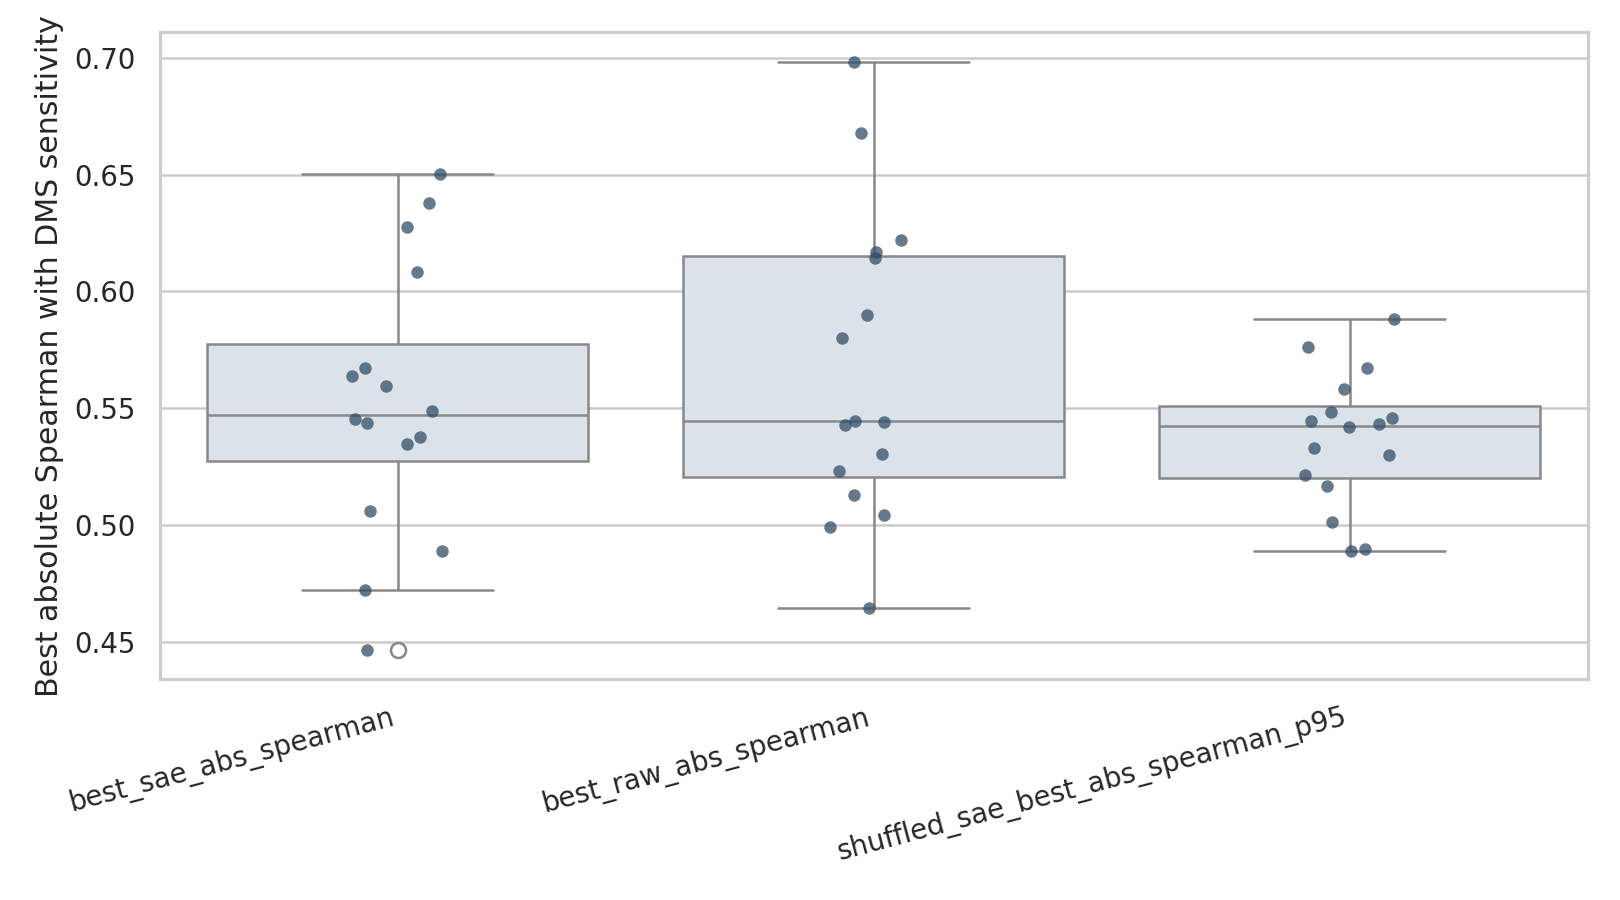
\includegraphics[width=0.95\linewidth]{figures/baseline_comparison.png}
    \caption{Aggregate baseline comparison across 16 \proteingym assays. Sparse features often correlate with residue-level \dms sensitivity, but the best \sae feature per assay is statistically indistinguishable from the strongest raw hidden dimension and from shuffled sparse-feature controls in this pilot.}
    \label{fig:baseline}
\end{figure}

\begin{table}[t]
\centering
\resizebox{\textwidth}{!}{%
\begin{tabular}{@{}lc@{}}
\toprule
\textbf{Metric} & \textbf{Result} \\
\midrule
Assays & 16 \\
Total single substitutions & 12,085 \\
Total residue positions & 688 \\
Median best \sae abs. Spearman with \dms & {\bf 0.547} \\
Median best raw hidden-dim abs. Spearman & 0.544 \\
Median shuffled \sae 95th percentile & 0.543 \\
\sae $>$ raw assays & 8 / 16 \\
\sae $>$ shuffled 95th percentile assays & 9 / 16 \\
Wilcoxon \sae $>$ raw $p$-value & 0.798 \\
Wilcoxon \sae $>$ shuffled 95th $p$-value & 0.217 \\
Median \esm score vs. \dms Spearman & 0.340 \\
\midrule
Best \sae median 95\% CI & [0.526, 0.578] \\
Best raw median 95\% CI & [0.523, 0.615] \\
\sae minus raw median 95\% CI & [-0.052, 0.027] \\
\sae minus shuffled median 95\% CI & [-0.025, 0.055] \\
\bottomrule
\end{tabular}
}
\caption{Aggregate performance across 16 \proteingym assays. Best absolute correlation is bolded, but paired tests and confidence intervals do not support a reliable aggregate \sae advantage over raw hidden dimensions or shuffled sparse controls.}
\label{tab:aggregate}
\end{table}


The bootstrap confidence intervals reinforce the same conclusion. The median best \sae correlation has 95\% CI 0.526--0.578, while raw hidden dimensions have 95\% CI 0.523--0.615 and shuffled controls have 95\% CI 0.522--0.552. The median \sae-minus-raw difference is $-0.0035$ with 95\% CI $[-0.052, 0.027]$, and the median \sae-minus-shuffled difference is 0.0089 with 95\% CI $[-0.025, 0.055]$. These intervals cross zero, so the aggregate data support feature triage but not a claim that sparse features are reliably better functional markers in this setting.

\para{Low-motif-alignment candidates are rare.} We next ask whether high-ranking feature-assay pairs remain after excluding features aligned with implemented motif scans. \Figref{fig:candidates} and \tabref{tab:candidates} show the three pairs that pass the low target-motif and low \swissprot motif-alignment heuristic. All three have zero target motif overlap among active positions and \swissprot motif AUROC close to 0.5. Their correlations with \dms sensitivity are moderate, with Spearman correlations from $-0.389$ to $-0.484$.

\begin{figure}[t]
    \centering
    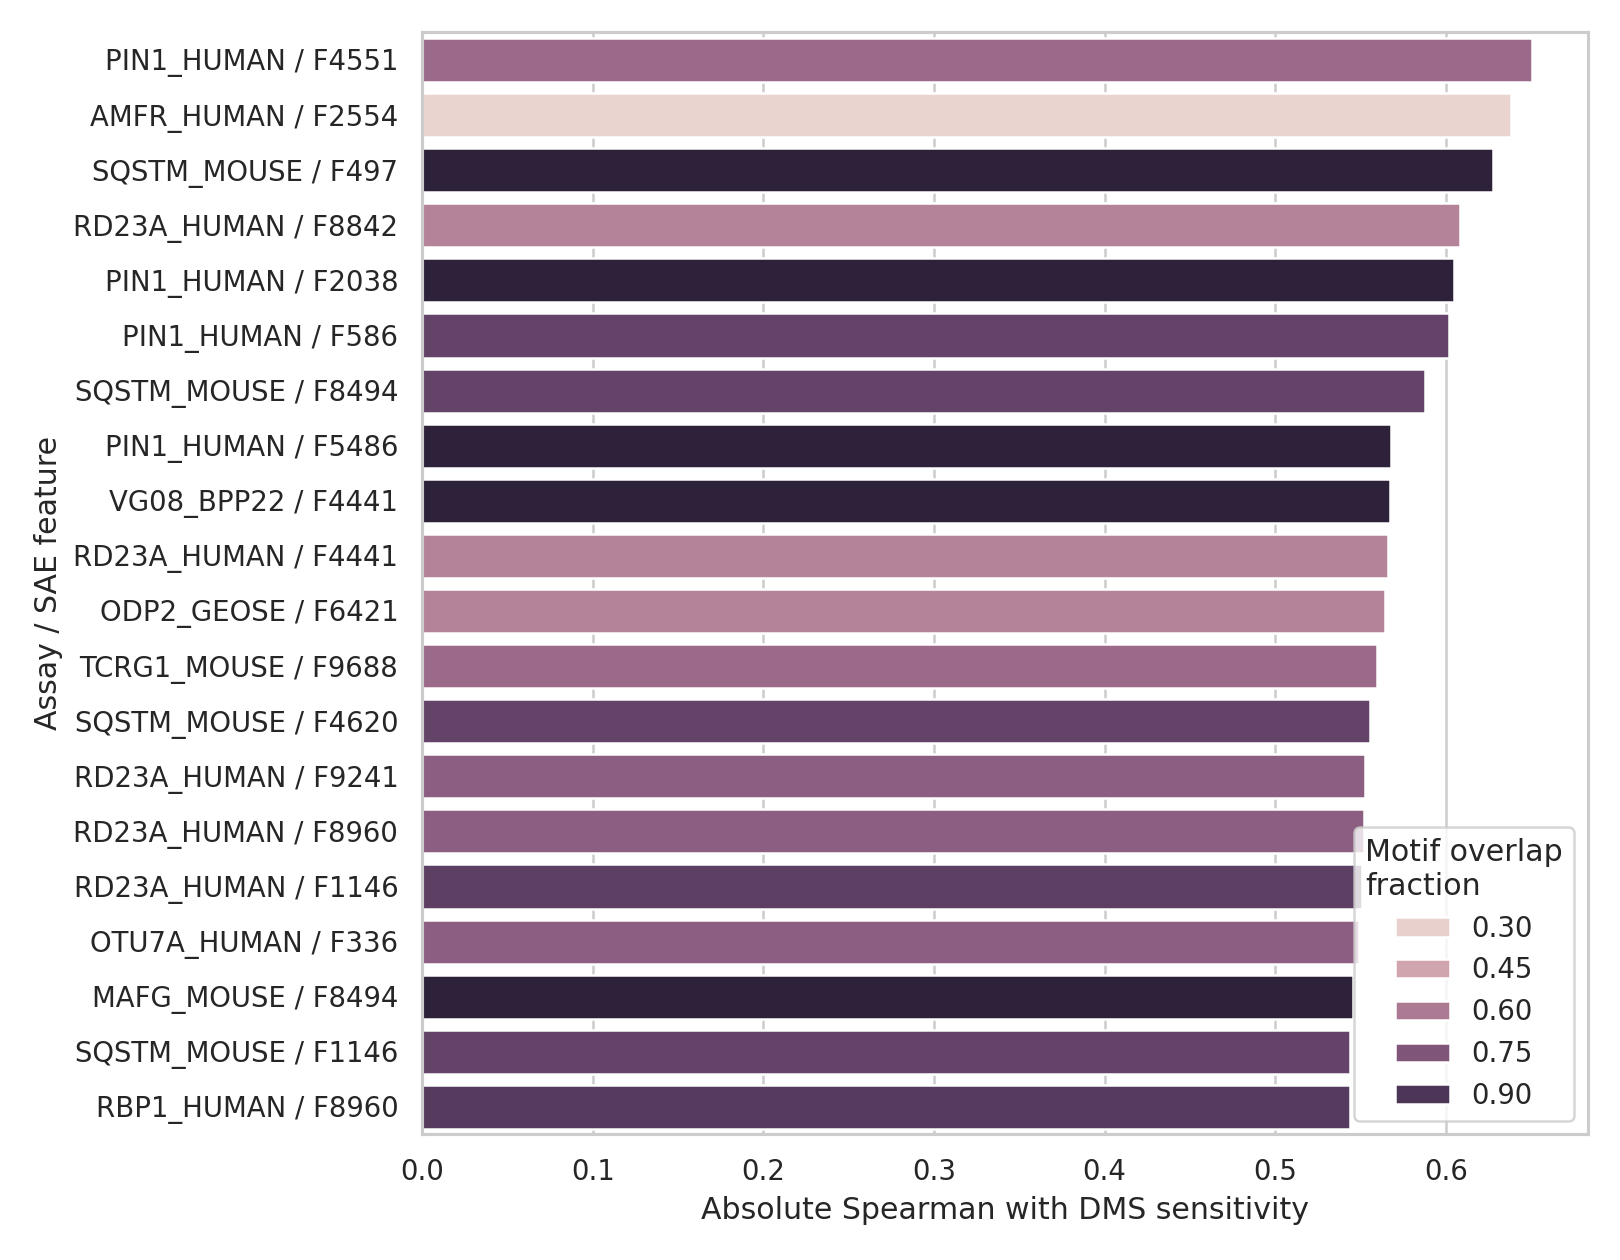
\includegraphics[width=0.95\linewidth]{figures/top_candidates.png}
    \caption{Top low-motif-alignment candidate features. The screen identifies three feature-assay pairs whose active target positions do not overlap the implemented \elm/\prosite motif scan and whose \swissprot motif AUROC is near random. These are candidate hypotheses, not discoveries, because feature-level FDR correction does not support significance.}
    \label{fig:candidates}
\end{figure}

\begin{table}[t]
\centering
\resizebox{\textwidth}{!}{%
\begin{tabular}{@{}lrrrrrr@{}}
\toprule
\textbf{Assay} & \textbf{Feature} & \textbf{Rank} & \textbf{\dms Spearman} & \textbf{\esm Spearman} & \textbf{Target overlap} & \textbf{\swissprot AUC} \\
\midrule
\texttt{TCRG1\_MOUSE\_Tsuboyama\_2023\_1E0L} & 7309 & 4 & {\bf -0.484} & -0.262 & 0.000 & 0.508 \\
\texttt{YNZC\_BACSU\_Tsuboyama\_2023\_2JVD} & 6419 & 5 & -0.400 & 0.028 & 0.000 & 0.486 \\
\texttt{TCRG1\_MOUSE\_Tsuboyama\_2023\_1E0L} & 7168 & 19 & -0.389 & -0.100 & 0.000 & 0.502 \\
\bottomrule
\end{tabular}
}
\caption{Low-motif-alignment candidate feature-assay pairs. All three have zero target motif overlap among active positions and near-random \swissprot motif AUROC. Best absolute \dms association is bolded.}
\label{tab:candidates}
\end{table}


The candidate table also shows why the novelty claim must remain conservative. All three candidates have Benjamini-Hochberg $q=1.0$ over the full feature set. This is expected under the limited 200-permutation budget and the 10,240 tested sparse features, but it means that nominal permutation $p$-values from 0.00498 to 0.0199 should be used only for ranking, not confirmatory inference.

\para{One candidate intervention changes masked-marginal scores.} We ablate the decoder directions for the selected candidates during \esm masked-marginal scoring. \Figref{fig:intervention} and \tabref{tab:interventions} report the high-minus-low activation effect. Two \texttt{TCRG1\_MOUSE\_Tsuboyama\_2023\_1E0L} candidates show negligible or non-significant differences. In contrast, feature 6419 in \texttt{YNZC\_BACSU\_Tsuboyama\_2023\_2JVD} changes mutation scores more at high-activation positions than low-activation positions, with an effect of 0.0223 log-prob units and Mann-Whitney $p=0.00495$.

\begin{figure}[t]
    \centering
    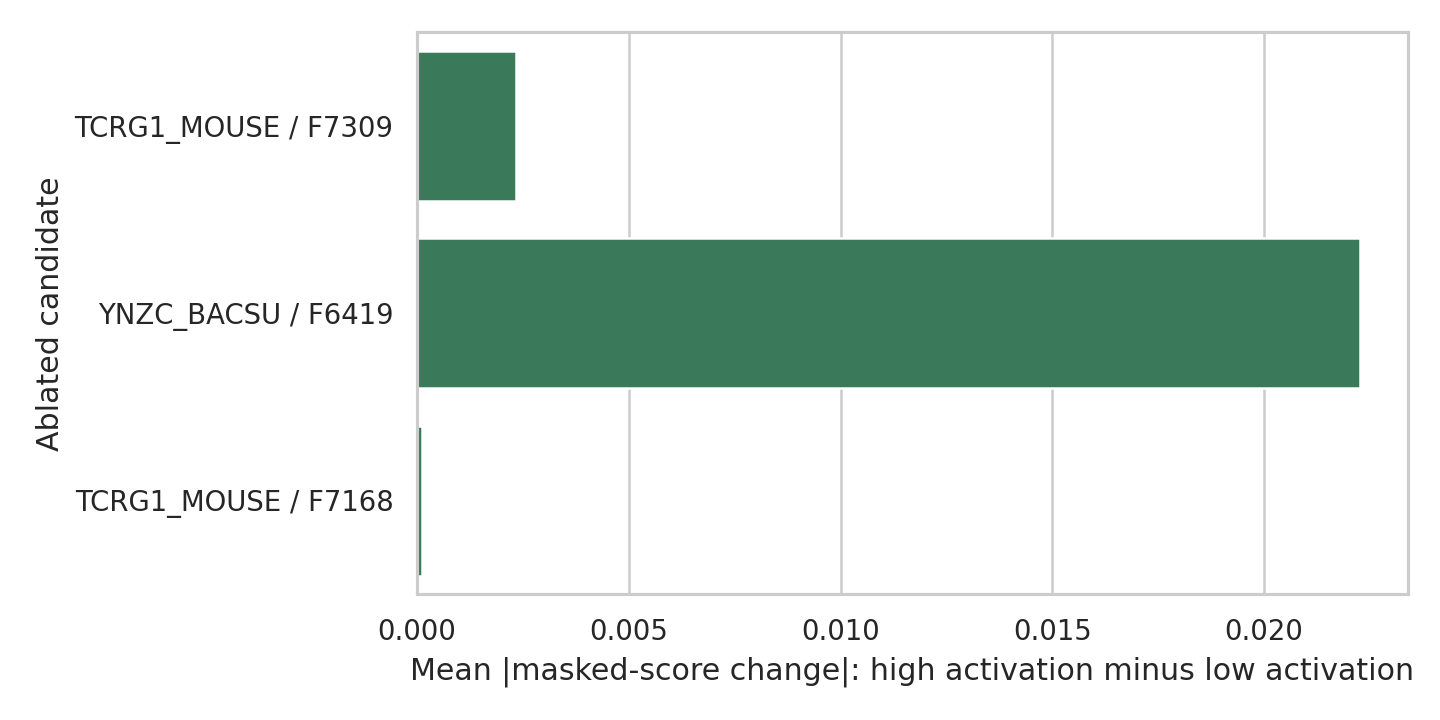
\includegraphics[width=0.95\linewidth]{figures/intervention_effects.png}
    \caption{Internal intervention effects for the three low-motif-alignment candidates. Ablating feature 6419 in the \texttt{YNZC\_BACSU} assay produces the clearest high-minus-low activation effect on masked-marginal mutation scores, while the two \texttt{TCRG1\_MOUSE} candidates do not show comparable separation.}
    \label{fig:intervention}
\end{figure}

\begin{table}[t]
\centering
\resizebox{\textwidth}{!}{%
\begin{tabular}{@{}lrrrrr@{}}
\toprule
\textbf{Assay} & \textbf{Feature} & \textbf{Mutations} & \textbf{Positions} & \textbf{High--low effect} & \textbf{Mann-Whitney $p$} \\
\midrule
\texttt{TCRG1\_MOUSE\_Tsuboyama\_2023\_1E0L} & 7309 & 621 & 35 & 0.00233 & 0.254 \\
\texttt{YNZC\_BACSU\_Tsuboyama\_2023\_2JVD} & 6419 & 714 & 39 & {\bf 0.02228} & {\bf 0.00495} \\
\texttt{TCRG1\_MOUSE\_Tsuboyama\_2023\_1E0L} & 7168 & 621 & 35 & 0.00013 & 0.498 \\
\bottomrule
\end{tabular}
}
\caption{Decoder-direction ablations for low-motif-alignment candidates. The effect is the mean absolute masked-score change at high-activation positions minus the corresponding change at low-activation positions. Best effect and smallest $p$-value are bolded.}
\label{tab:interventions}
\end{table}


Feature 6419 is therefore the strongest follow-up candidate in this run. The result is causal with respect to the model computation, because modifying the feature direction changes masked-marginal scores. It is not yet causal with respect to biology. The intervention was selected after screening, the effect is measured in model log-probability units rather than experimental fitness, and the feature does not strongly correlate with \esm residue sensitivity. We treat it as an exploratory candidate for structural or biochemical follow-up.
